% **************************************************************************************************************
% A Classic Thesis Style
% An Homage to The Elements of Typographic Style
%
% Copyright (C) 2015 André Miede http://www.miede.de
%
% If you like the style then I would appreciate a postcard. My address 
% can be found in the file ClassicThesis.pdf. A collection of the 
% postcards I received so far is available online at 
% http://postcards.miede.de
%
% License:
% This program is free software; you can redistribute it and/or modify
% it under the terms of the GNU General Public License as published by
% the Free Software Foundation; either version 2 of the License, or
% (at your option) any later version.
%
% This program is distributed in the hope that it will be useful,
% but WITHOUT ANY WARRANTY; without even the implied warranty of
% MERCHANTABILITY or FITNESS FOR A PARTICULAR PURPOSE.  See the
% GNU General Public License for more details.
%
% You should have received a copy of the GNU General Public License
% along with this program; see the file COPYING.  If not, write to
% the Free Software Foundation, Inc., 59 Temple Place - Suite 330,
% Boston, MA 02111-1307, USA.
%
% **************************************************************************************************************
% arara: pdflatex
% arara: bibtex
% arara: bibtex: { files: [ JDHV ] }
% arara: pdflatex
% arara: pdflatex
\RequirePackage{fix-cm} % fix some latex issues see: http://texdoc.net/texmf-dist/doc/latex/base/fixltx2e.pdf
\documentclass[ oneside,openright,titlepage,numbers=noenddot,headinclude,%1headlines,% letterpaper a4paper
                footinclude=false,cleardoublepage=empty,abstractoff, % <---
                % obsolete, remove (todo)
                BCOR=5mm,paper=a4,fontsize=11pt,%11pt,a4paper,%
                ngerman,american,%
                ]{scrreprt}

%********************************************************************
% Note: Make all your adjustments in here
%*******************************************************
\input{classicthesis-config}

%********************************************************************
% Bibliographies
%*******************************************************
\addbibresource{0_frontmatter/PhDThesis.bib}


%********************************************************************
% Hyphenation
%*******************************************************
%\hyphenation{put special hyphenation here}

% ********************************************************************
% GO!GO!GO! MOVE IT!
%*******************************************************
\DeclareMathOperator*{\argmin}{arg\,min}
\DeclareMathOperator*{\argmax}{arg\,max}

\begin{document}
\frenchspacing
\raggedbottom
\selectlanguage{american} % american ngerman
\pagenumbering{roman}
\pagestyle{plain}
%********************************************************************
% Frontmatter
%*******************************************************
%*******************************************************
% Titlepage
%*******************************************************
\begin{titlepage}
    % if you want the titlepage to be centered, uncomment and fine-tune the line below (KOMA classes environment)
    %\begin{addmargin}[-1cm]{-3cm}
    \begin{center}
        \large  

        \hfill

        \vfill

        \includegraphics[width=10cm]{0_frontmatter/figures/udg_logo} \\ \medskip
        
        %\vfill
        \myDegree \\ \bigskip

        \begingroup
            \spacedallcaps{\myTitle} \\ \bigskip
        \endgroup

        \spacedlowsmallcaps{\myName} \\ \bigskip

        %\mySubtitle \\ \medskip   
        %\myDepartment \\                            
        %\myFaculty \\
        %\myUni \\ \bigskip

        \myTime%\ -- \myVersion

        \vfill                      

    \end{center}  
  %\end{addmargin}       
\end{titlepage}   
\include{0_frontmatter/Titleback}
%*******************************************************
% Titlepage
%*******************************************************
\begin{titlepage}
    % if you want the titlepage to be centered, uncomment and fine-tune the line below (KOMA classes environment)
    %\begin{addmargin}[-1cm]{-3cm}
    \begin{center}
        \large  

		\hfill
		\vfill
		
		\includegraphics[width=10cm]{0_frontmatter/figures/udg_logo} \\ \medskip
	
        \hfill

        %\vfill

		\myDegree \\ \bigskip
		
        \begingroup
            \color{Maroon}\spacedallcaps{\myTitle} \\ \bigskip
        \endgroup

        \spacedlowsmallcaps{\myName}

        \vfill

        \myTime \\ \medskip
        Doctoral Program in Technology\\ \bigskip
        \textit{Supervised by:}\\
        
        \mySupervisor and \myOtherSupervisor \\ \bigskip
        
        Thesis submitted to the University of Girona in fulfillment of the
        requirements for the degree of Doctor of Philosophy

        %\mySubtitle \\ \medskip   
        %\myDegree \\
        %\myDepartment \\                            
        %\myFaculty \\
        %\myUni \\ \bigskip

        \vfill                      

    \end{center}  
  %\end{addmargin}       
\end{titlepage}   

\include{0_frontmatter/Titleback}
\cleardoublepage
%*******************************************************
% Declaration
%*******************************************************
\refstepcounter{dummy}
\pdfbookmark[0]{CERTIFICAT DE DIRECCIO DE TESI}{Certificat de Direccio de Tesi}
\chapter*{Certificat de Direcció de Tesi}
\thispagestyle{empty}

Dr. Pere Vilà Talleda and Dr. Lluís Fàbrega Soler, del Departament 
d’Arqui-tectura i Tecnologia de Computadors de la Universitat de Girona,

\bigskip

DECLAREM:

\bigskip

\noindent Que el treball titulat \myTitle, que presenta \myName per a l’obtenció
del títol de doctor, ha estat realitzat sota la nostra direcció i que compleix els requisits
per poder optar a Menció Internacional.

\bigskip

I, perquè així consti i tingui els efectes oportuns, signem aquest
document.

\bigskip
 
\noindent\textit{Girona, Juliol 2018}

\smallskip

\begin{flushright}
    \begin{tabular}{m{5cm} m{1.5cm} m{5cm}}
        \\ \cline{1-1} \cline{3-3}
        \centering\mySupervisor& &\centering\myOtherSupervisor \\
    \end{tabular}
\end{flushright}

\include{0_frontmatter/Titleback}
%*******************************************************
% Acknowledgments
%*******************************************************
\pdfbookmark[1]{Acknowledgments}{acknowledgments}

\bigskip

\begingroup
\let\clearpage\relax
\let\cleardoublepage\relax
\let\cleardoublepage\relax
\chapter*{Acknowledgments}


\endgroup




\include{0_frontmatter/Titleback}
%*******************************************************
% Publications
%*******************************************************
\pdfbookmark[1]{Publications}{publications}
\chapter*{Publications}%\graffito{This is just an early --~and currently ugly~--
% test!}
\label{sec:publications}

The work developed in this thesis led to the following publications:

\section*{JOURNAL ARTICLES}
\begin{enumerate}[{[1]}]
  \item \textbf{D. Aguirre-Guerrero}, M. Camelo, P. Vil\`a and Ll. F\`abrega, 
  "WMGR: A Generic and Compact Routing Scheme for Data Center Networks," in
  \textit{IEEE/ACM Transactions on Networking}, vol. 26, no. 1, pp. 356-369. Feb. 2018.
  DOI: 10.1109/TNET.2017.2779866
\end{enumerate}

\section*{PEER-REVIEWED CONFERENCES AND WORKSHOPS}
\begin{enumerate}[{[1]}]
  \item \textbf{D. Aguirre-Guerrero}, M. Camelo, P. Vil\`a and Ll. F\`abrega, 
  "Compact Greedy Routing in Large-scale Networks using Word-metric Spaces,"
  \textit{1st. International Workshop on Elastic Networks Design and Optimization},
  Cartagena, Spain, 2016.
\end{enumerate}


\section*{OTHER CONFERENCES AND WORKSHOPS}

\begin{enumerate}[label={[\arabic*]}]
  \item \textbf{D. Aguirre-Guerrero}, P. Vil\`a and Ll. F\`abrega, 
  "Encaminamiento de Informaci{\'o}n en Redes Comunicaci{\'o}n de Gran Escala,"
  \textit{6to. Simposio de Becarios CONACyT en Europa}, Strasbourg, France 2017.
  \item \textbf{D. Aguirre-Guerrero}, P. Vil\`a and Ll. F\`abrega, 
  "Greedy Geometric in Word Metric Spaces,"
  \textit{1st. Conference of Pre-doctorals Researches}, Girona, Spain, 2016. 
  ISBN: 978-8-48458-502-2
\end{enumerate}

\pagestyle{scrheadings}
\cleardoublepage
\include{0_frontmatter/Contents}
\include{0_frontmatter/Titleback}
%*******************************************************
% Abstract
%*******************************************************
%\renewcommand{\abstractname}{Abstract}
\pdfbookmark[1]{Abstract}{Abstract}
\begingroup
\let\clearpage\relax
\let\cleardoublepage\relax
\let\cleardoublepage\relax

\chapter*{Abstract}

Since \ac{WMGR}  \textit{a priori} (\eg exploring confined
natural environments like underwater caves). In these scenarios, \acp{WMGR} 
\vfill

\endgroup			

\vfill

\include{0_frontmatter/Titleback}
%*******************************************************
% Abstract
%*******************************************************
%\renewcommand{\abstractname}{Abstract}
\pdfbookmark[1]{Resumen}{Resumen}
\begingroup
\let\clearpage\relax
\let\cleardoublepage\relax
\let\cleardoublepage\relax

\chapter*{Resumen}

Desde sus inicios a finales de los años 50, las capacidades y aplicaciones de
los vehículos autónomos submarinos o AUVs (por sus siglas en inglés) han estado
bajo un continuo proceso de evolución. Las aplicaciones más comunes incluyen la
obtención de imágenes e inspeccción de diferentes tipos de estructuras, tales
como cascos de barcos, estructuras naturales en el fondo marino, así como la
recolección de información oceanográfica como datos biológicos, químicos e
incluso arqueológicos.

Muchas de estas aplicaciones requieren información \textit{a priori} del área o
estructura que va a ser inspeccionada, ya sea para navegar a una altitud segura
o para precalcular un camino para realizar estudios, el cual puede ser corregido
o modificado en tiempo real. Sin embargo, existen aplicaciones similares o nuevas,
como la exploración de entornos naturales confinados (\eg cuevas submarinas),
donde dicha información puede no estar disponible. En estos escenarios, los AUVs
debe operan en entornos desconocidos, y por lo tanto los AUVs están más
expuestos a colisiones.

Aunque estas aplicaciones de AUVs comparten algunos requiremientos comunes con
otras aplicaciones de robots aéreos y terrestres (\eg localización, mapeo,
visión, etc.), navegar autónomamente mientras se ejecutan este tipo de tareas en
entornos submarinos difiere en ciertos factores, como la presencia de
pertubaciones externas (corrientes), bajo rango de visibilidad y limitaciones en
la precisión del sistema de navegación. Para poder abordar dichas restricciones
se requiere un planificador de movimientos con capacidad de cómputo en tiempo
real, el que contribuya a superar las limitaciones en la información del entorno
y la falta de precisión de posicionamiento, en especial cuando se navega cerca
de los obstáculos de su alrededor.

En este sentido, esta tesis presenta una método para dotar un AUV con la
habilidad para moverse a través de entornos no explorados. Para ello, esta tesis
propone un método para calcular en tiempo real caminos factibles y seguros. El
método propuesto permite al vehículo construir incrementalmente un mapa del
entorno, y al mismo tiempo replaninficar el camino factible hacia la meta u
objetivo establecido. Para lograr esto, es necesario considerar las
restricciones de movimiento para planificar caminos 2D y 3D que sean factibles o
realizables.

Para evaluar el método propuesto, se realizaron diferentes experimentos con los
AUVs Sparus~II y AsterX, ambos vehículos tipo torpedo que realizaron
misiones de manera autónoma en diferentes escenarios. Estos experimentos
incluyen pruebas en simulación y en el agua en diferentes entornos, tales como
estructuras marinas artificiales, estructuras marinas naturales, así entornos
naturales confinados.

\vfill

% \begin{otherlanguage}{ngerman}
% \pdfbookmark[1]{Zusammenfassung}{Zusammenfassung}
% \chapter*{Zusammenfassung}
% Kurze Zusammenfassung des Inhaltes in deutscher Sprache\dots 
% \end{otherlanguage}

\endgroup			

\vfill
\include{0_frontmatter/Titleback}
%*******************************************************
% Abstract
%*******************************************************
%\renewcommand{\abstractname}{Abstract}
\pdfbookmark[1]{Resum}{Resum}
\begingroup
\let\clearpage\relax
\let\cleardoublepage\relax
\let\cleardoublepage\relax

\chapter*{Resum}

Des dels inicis a finals dels anys 50, les capacitats i aplicacions dels
vehicles autònoms submarins o AUVs (per les seves sigles en anglès) han
experimentat un procés d'evolució continu. Les aplicacions més comunes són
l’obtenció d'imatges i inspecció de diferents tipus d'estructures, com per
exemple, cascos de vaixells o estructures naturals en el fons marí, i
l'adquisició d'informació oceanogràfica com dades biològiques, químiques i
arqueològiques.

Moltes d'aquestes aplicacions requereixen informació \textit{a priori} de l'àrea
o estructura que es vol inspeccionar, ja sigui per navegar a una altitud segura
o per calcular en avançat un camí que permeti realitzar els estudis, el qual pot
ser corregit o modificat a temps real. No obstant, existeixen aplicacions
similars o noves, com l'exploració d'entorns naturals confinats (\eg coves
submarines), on aquesta informació pot ser inexistent. En aquests casos, els
AUVs han d'operar en entorns desconeguts, pel que estan més exposats a
col·lisions.

Tot i que aquestes aplicacions de AUVs comparteixen alguns requeriments comuns
amb altres aplicacions de robots aeris i terrestres (\eg localització, mapeig,
visió, etc.), navegar autònomament al mateix temps que s'executen aquest tipus
de tasques en entorns submarins difereix en certs factors, com la presencia de
pertorbacions externes (corrents), baix rang de visibilitat i limitacions en la
precisió del sistema de navegació. Per poder tractar les esmentades restriccions
és necessari un planificador de moviments amb capacitat de processament en temps
real, el que ajudi a superar les limitacions en la informació de l'entorn i la
falta de precisió de posicionament, en especial quan es navega a prop dels
obstacles presents en el seu voltant.

En aquest sentit, aquesta tesis presenta una alternativa per dotar un AUV amb
l'habilitat de moure’s a través d'entorns no explorats. Per aconseguir aquesta
fita, aquesta tesis proposa un mètode per calcular en temps real camins
factibles i segurs. El mètode proposat permet al vehicle construir de forma
incremental un mapa de l'entorn, i al mateix temps replanificar un camí factible
cap a l'objectiu establert. Per assolir això, el mètode proposat te en compte
les restriccions de moviment del vehicle per planificar camins 2D i 3D que
siguin factibles o realitzables.

Per avaluar el mètode proposat, s'han realitzat diferents experiments amb els
AUVs Sparus~II i l'AsterX, els quals són vehicles de tipus torpede que van
realitzar missions de forma autònoma en diferents escenaris. Aquests experiments
inclouen proves en simulació i a l'aigua en diferents entorns, tal i com
estructures marines artificials, estructures marines naturals i entorns naturals
confinats.


\vfill

% \begin{otherlanguage}{ngerman}
% \pdfbookmark[1]{Zusammenfassung}{Zusammenfassung}
% \chapter*{Zusammenfassung}
% Kurze Zusammenfassung des Inhaltes in deutscher Sprache\dots 
% \end{otherlanguage}

\endgroup			

\vfill
\include{0_frontmatter/Titleback}
%********************************************************************
% Mainmatter
%*******************************************************
\cleardoublepage\pagenumbering{arabic}
\cleardoublepage
\acresetall

%*******************************************************
% Part I
%*******************************************************
\ctparttext{You can put some informational part preamble text here. Illo principalmente su nos. Non message \emph{occidental} angloromanic da. Debitas effortio simplificate sia se, auxiliar summarios da que, se avantiate publicationes via. Pan in terra summarios, capital interlingua se que. Al via multo esser specimen, campo responder que da. Le usate medical addresses pro, europa origine sanctificate nos se.} % Text on the Part 1 page describing  the content in Part 1

\part{Preliminaries} % First part of the thesis
%*******************************************************

\include{1_introduction/1_introduction}
\cleardoublepage
% this file is called up by thesis.tex
% content in this file will be fed into the main document

\chapter{Theoretical Framework} % top level followed by section, subsection
\label{ch:theo_frame}
%************************************************

% the code below specifies where the figures are stored
\ifpdf
    \graphicspath{{2_preliminaries/figures/PNG/}{2_preliminaries/figures/PDF/}{2_preliminaries/figures/}}
\else
    \graphicspath{{2_preliminaries/figures/EPS/}{2_preliminaries/figures/}}
\fi

% ----------------------------------------------------------------------
%: ----------------------- preliminaries content ----------------------- 
% ----------------------------------------------------------------------



%: ----------------------- HELP: latex document organisation
% the commands below help you to subdivide and organise your thesis
%    \chapter{}       = level 1, top level
%    \section{}       = level 2
%    \subsection{}    = level 3
%    \subsubsection{} = level 4
% note that everything after the percentage sign is hidden from output

%: ----------------------- section: Graph Theory ----------------------- 

\section{Graph Theory}

%: ----------------------- section: Finite State Automata ----------------------- 

\section{Finite State Automata}

\subsection{Regular Languages}

\subsection{2-variable Finite State Automata}

\subsection{Existential Quantification}

%: ----------------------- section: Group Theory ----------------------- 

\section{Group Theory}

\subsection{Finitely Presented Groups}

\subsection{Group Homomorphism}

\subsection{Abelian Groups}

\subsection{Cayley Graphs}

%: ----------------------- section: Automatic Groups ----------------------- 

\section{Automatic Groups}

\subsection{Automatic Structures}

\subsection{Words as Nodes and Paths}

\subsection{Solving the Shortest Path Problem in Cayley Graphs}

\cleardoublepage
% this file is called up by thesis.tex
% content in this file will be fed into the main document

\chapter{Cayley Graphs: Applications and Routing Algorithms} % top level followed by section, subsection
\label{ch:cg_app_routing}
%************************************************

% the code below specifies where the figures are stored
\ifpdf
    \graphicspath{{3_cg_app_routing/figures/PNG/}{3_cg_app_routing/figures/PDF/}{3_cg_app_routing/figures/}}
\else
    \graphicspath{{3_cg_app_routing/figures/EPS/}{3_cg_app_routing/figures/}}
\fi

% ----------------------- contents from here ------------------------

\section{Topological Properties of Cayley Graphs}
\section{Applications}
\subsection{Interconnection Networks}
\subsubsection{Processor Interconnection Networks}
\subsubsection{Data Center Networks}
\subsubsection{Wireless Sensor Networks}
\subsection{Error Correcting Codes}
\subsection{Hash Functions}
\section{Routing Algorithms}
\subsection{Performance Metrics}
\subsection{Sims Factoring Algorithm}
\subsection{Permutation-sort Algorithm}
\subsection{Routing Algorithm for Boreal Cayley Graphs}
% ---------------------------------------------------------------------------
% ----------------------- end of thesis sub-document ------------------------
% ---------------------------------------------------------------------------

\cleardoublepage

%*******************************************************
% Part II
%*******************************************************
\ctparttext{You can put some informational part preamble text here. Illo principalmente su nos. Non message \emph{occidental} angloromanic da. Debitas effortio simplificate sia se, auxiliar summarios da que, se avantiate publicationes via. Pan in terra summarios, capital interlingua se que. Al via multo esser specimen, campo responder que da. Le usate medical addresses pro, europa origine sanctificate nos se.} % Text on the Part 1 page describing  the content in Part II

\part{Word-Metric-based Greedy Routing} % First part of the thesis
%*******************************************************

% this file is called up by thesis.tex
% content in this file will be fed into the main document

%: ----------------------- name of chapter  -------------------------
\chapter{Path Computation in Cayley Graphs}
\label{ch:path_comp_in_cg} %
% top level followed by section, subsection


%: ----------------------- paths to graphics ------------------------

% change according to folder and file names
\ifpdf
    \graphicspath{{4_path_comp_in_cg/figures/PNG/}{4_path_comp_in_cg/figures/PDF/}{4_path_comp_in_cg/figures/}}
\else
    \graphicspath{{4_path_comp_in_cg/figures/EPS/}{4_path_comp_in_cg/figures/}}
\fi

%: ----------------------- contents from here ------------------------

\section{Distributed Configuration}

\subsection{Memory Space Requirements}

\section{Computing the Shortest Path}

\section{Computing the $K$-Shortest Paths}

\section{Computing the Shortest Node-disjoint Shortest Paths}

\section{Computing the Shortest Edge-disjoint Shortest Paths}

% ---------------------------------------------------------------------------
%: ----------------------- end of thesis sub-document ------------------------
% ---------------------------------------------------------------------------


\cleardoublepage
% this file is called up by thesis.tex
% content in this file will be fed into the main document

%: ----------------------- name of chapter  -------------------------
\chapter{Fault-tolerant Routing in Cayley Graphs}
\label{ch:fault_tolerant}
% top level followed by section, subsection


%: ----------------------- paths to graphics ------------------------

% change according to folder and file names
\ifpdf
    \graphicspath{{5_fault_tolerant/figures/PNG/}{5_fault_tolerant/figures/PDF/}{5_fault_tolerant/figures/}}
\else
    \graphicspath{{5_fault_tolerant/figures/EPS/}{5_fault_tolerant/figures/}}
\fi

%: ----------------------- contents from here ------------------------

\section{Multiple-node Failures}

\subsection{Computing the Shortest Path Avoiding a Set of Nodes}

\subsection{Node-failure Notification}

\subsection{Node-failure Recovery}

\section{Multiple-edge Failures}

\subsection{Computing the Shortest Path Avoiding a Set of Edges}

\subsection{Edge-failure Notification}

\subsection{Edge-failure Recovery}



% ---------------------------------------------------------------------------
%: ----------------------- end of thesis sub-document ------------------------
% ---------------------------------------------------------------------------


\cleardoublepage
% this file is called up by thesis.tex
% content in this file will be fed into the main document

%: ----------------------- name of chapter  -------------------------
\chapter{Performance Evaluation}
\label{ch:performance_evaluation} % top level followed by section,
% subsection


%: ----------------------- paths to graphics ------------------------

% change according to folder and file names
\ifpdf
    \graphicspath{{6_performance_evaluation/figures/PNG/}{6_performance_evaluation/figures/PDF/}{6_performance_evaluation/figures/}}
\else
    \graphicspath{{6_performance_evaluation/figures/EPS/}{6_performance_evaluation/figures/}}
\fi

%: ----------------------- contents from here ------------------------
\section{Stretch}

\section{Space Requirements}

 \subsection{Node Label}

    \subsubsection{Source Routing}

    \subsubsection{Hop-by-hop Routing}

  \subsection{Automatic Structures}

\section{Forwarding Desicion Time}

    \subsection{Source Routing}

    \subsection{Hop-by-hop Routing}

\section{Convergence Time of Fault-tolerant Rounting}

\section{Message Complexity}

    \subsection{Node Label Assigment}

    \subsection{Failures Notification}

    \subsection{Recovery Notification}

% ---------------------------------------------------------------------------
%: ----------------------- end of thesis sub-document ------------------------
% ---------------------------------------------------------------------------


\cleardoublepage
% this file is called up by thesis.tex
% content in this file will be fed into the main document

\chapter{Conclusions}\label{ch:conclusions} % top level followed by section,
% subsection


% ----------------------- paths to graphics ------------------------

% change according to folder and file names
\ifpdf
    \graphicspath{{7_conclusions/figures/PNG/}{7_conclusions/figures/PDF/}{7_conclusions/figures/}}
\else
    \graphicspath{{7_conclusions/figures/EPS/}{7_conclusions/figures/}}
\fi


% ----------------------- contents from here ------------------------


\section{Summary of Completed Work}

This thesis has addressed the problem of planning paths online for an \acf{AUV},
which navigates under motion constraints through unexplored environments. This
kind of missions require the vehicle to incrementally map the surroundings,
while simultaneously replanning a feasible and safe path. After providing an
overview of the general problem and the proposed objectives to tackle it,
Chapter~\ref{ch:state_of_the_art} presented the state of the art of path/motion
planning for robotic systems. This review started with discussing the general
planing problem, then it classified the available techniques, and finally it
discussed their most common extensions. For this latter part, the review put
special emphasis on those methods that have been used with underwater vehicles.

Chapter~\ref{ch:motion_constratins} presented the use of sampling-based methods
to plan feasible and constant-depth paths for a torpedo-shaped \ac{AUV}.
Here the term feasible refers to paths that take into consideration the
vehicle's limitations, either kinematic or dynamic ones. In the case analysed in
this thesis, torpedo-shaped \acp{AUV} are kinematically constrained, since they
cannot conduct pure lateral motion. Instead, they are required to move forward
or backward while conducting turning maneuvers. Two different approaches to
consider such limitations were presented and discussed. The first one directly
uses the \ac{AUV} kinematic equation of motion. The second one employs Dubins
curves to characterize the \ac{AUV} motion with straight line segments and
circular arcs. Both approaches were evaluated and compared in different
simulations. This allowed identifying their advantages and drawbacks, which led
to establish the one using Dubins curves as the best approach.

Chapter~\ref{ch:planning_3D} proposed an alternative formulation to plan
feasible and variable-depth paths for a torpedo-shaped \ac{AUV}. This
formulation extended the Dubins curves by including the \ac{AUV} vertical
motion, and it was also used with a sampling-based planning method. This sought
to define a general strategy to plan \ac{3D} paths, which took into account both
the vehicle's lateral and vertical motion constraints. This approach was
evaluated in different simulated scenarios, where it was compared with another
approach that does not include the vehicle's motion constraints involved.
Results proved that the proposed approach allows an \ac{AUV} to follow more
accurately \ac{3D} paths.

While simulation tests in Chapters~\ref{ch:motion_constratins} and
\ref{ch:planning_3D} assumed fully mapped environments, the main objective of
this thesis was to endow an \ac{AUV} with the capability to move through
unexplored environments. In order to do so, Chapter~\ref{ch:plann_online}
introduced an online mapping and path/motion planning framework for \acp{AUV}.
The framework uses an Octomap to incrementally build a representation of the
surroundings. To calculate the \ac{AUV} path, it includes a sampling-based
planner that employs the extended Dubins curves formulation for dealing with
\ac{2D} and \ac{3D} missions. Furthermore, the planner not only computes a
feasible path, but also attempts to obtain a safe one by minimizing its
associated risk. Finally, the framework incorporates new strategies that seek to
reduce the running time, which is a critical requirement for the intended
applications and their online computation limitations. The framework was
evaluated with simulations in different scenarios.

In order to completely validate the proposed framework and its properties,
Chapter~\ref{ch:applications} presented different experiments that were
conducted by torpedo-shaped \acp{AUV}. This included four different real-world
scenarios:

\begin{inparaenum}[1)]
\item \textit{Planning constant-depth paths to move through artificial marine
structures}. In this case, the Sparus~II \ac{AUV} traversed multiple times a
breakwater structure, which is composed of a series of concrete blocks separated
by four-meter gaps. At the beginning of the mission, the vehicle was not
provided with a map of the surroundings. This required the vehicle to
incrementally build a map, while planning a feasible and safe path to the
different specified goals. Furthermore, the vehicle was equipped with optical
cameras to gather images, which were used to create a \ac{3D} reconstruction of
the traveled area.

\item \textit{Planning constant-depth paths to move through natural marine
structures.} In this case, the Sparus~II navigated through a natural underwater
canyon made by rocky formations. This experiment sought to prove the
framework's capabilities in a more challenging scenario with non-regular shape
obstacles. As occurred in the previous experiment, the vehicle was not provided
with an initial map of the area, and it was also equipped with optical cameras.
The result of the mission also included a photo-realistic \ac{3D} reconstruction
of the natural scenario.

\item \textit{Planning variable-depth paths to move through confined marine
environments.} In the previously mentioned experiments, the vehicle navigated at
a constant depth due to a sensor limitation. However, in order to validate the
capability to plan \ac{3D} paths, a simulated Sparus~II conducted missions over
a real-world dataset of a cave complex. This scenario required solving
consecutive start-to-goal queries of different depths. As occurred with the
previous experiments, the vehicle was not provided with an initial map of the
surroundings.

\item \textit{The autonomous survey replanning for gap filling and target
inspection.} In this case, the AsterX \ac{AUV} conducted an inspection of an
area of interest. The mission was composed of two phases. The first one required
the \ac{AUV} to follow a preplanned coverage path. The second one guided the
vehicle to further inspect either potential targets or gaps (\ie areas not
correctly covered). For this latter phase, the extended Dubins curves
formulation was used to plan \ac{3D} paths to guide the \ac{AUV} closer from the
potential targets. This experiment sought to complement the validation of
planning \ac{3D} paths with a real-world vehicle.
\end{inparaenum}

These tests allowed proving the viability of the proposed approach under
real-world conditions. This included the assessment of the computational
efficiency, in which a single embedded computer was capable of conducting
simultaneously mapping, planning, and control tasks. Furthermore, along the
development of the proposed framework, the success rate increased from $10-20\%$
during the initial tests, to $80-90\%$ when using the final version of the
framework. However, it is also important to mention that those failing cases
were mainly due to sensor limitations.

\section{Review of Contributions}

Aiming to endow \acp{AUV} with the capabilities required to operate in
unexplored environments, this thesis has proposed an online mapping and
path/motion planning framework. This led to extend and develop different
strategies that contribute to the current state-of-the-art for underwater
vehicles. Such contributions have been presented and peer-reviewed along
different~\nameref{sec:publications}, and they can be gathered in four main
aspects:

\begin{description}

\item[Path/Motion Planning online] This thesis established that in order to move
through unexplored environments, an \ac{AUV} has to be capable of incrementally
mapping the surroundings, while simultaneously planning collision-free paths.
However, an initial approach in this thesis was to have two vehicles to conduct
missions in unexplored environments. The first vehicle had to navigate at a safe
altitude, and it was assumed to be equipped with a downward-looking multibeam
sonar that allowed to build online a map. Such a map was used to simultaneously
plan collision-free paths for a second vehicle that navigated in close-proximity
to the sea bottom~[NGCUV'15]. Although the previous approach was limited to
simulation tests, it did contribute to define a first mechanism for simultaneous
mapping and planning~[OCEANS'15]. This mechanism later became the framework
thoroughly explained in Chapter~\ref{ch:plann_online}. In its first version, the
framework used an anytime tree-pruning strategy that \textit{opportunistically
check} states for collision~[ICRA'15], but it was later improved by
\textit{reusing the last best known solution}~[IROS'16].

\item[Planning feasible motion for AUVs] Although a simultaneous mapping and
planning mechanism allowed an \ac{AUV} to move through an unexplored
environment~[ICRA'15], results also showed multiple replanning maneuvers.
The main reason was that the \ac{AUV} was not capable of accurately following
the provided paths. This thesis identified the necessity to plan not only
collision-free paths, but also feasible ones. This means that the calculated
paths must take into consideration the vehicle's motion constraints, thus
minimizing unexpected vehicle's trajectories when attempting to follow the
calculated path. This thesis proposed and validated the use of Dubins curves to
characterize the constant-depth \ac{AUV} motions~[IROS'16], which was later
extended to consider full \ac{3D} trajectories~[JFR'17].

\item[Planning safe paths] \acp{AUV} operate in complex environments, where
they can be affected by external perturbations such as waves and currents.
Furthermore, \acp{AUV}' navigation system has a position error that cannot be
corrected while submerged, especially in environments where a mother ship
cannot be used with an \ac{USBL} system. These operation conditions can lead the
vehicle to risky situations, especially when moving in close-proximity to nearby
obstacles. This thesis evaluated different alternatives to plan not only
collision-free and feasible paths, but also ones that attempt to minimize the
risk of collision. A first alternative was to maintain a safe distance from the
surroundings~[NGCUV'15]. However, it was later replaced with an optimization
function that combines the length and the risk associated with a calculated
path~[IROS'16].

\item[Experimental Evaluation] This thesis has extensively proved the proposed
framework and its newly introduced capabilities. This validation mainly involved
the Sparus~II \ac{AUV}. The experiments included simulated and in-water trials
in different scenarios, such as artificial marine structures
(breakwater)~[ICRA'15, IROS'16], natural marine structures (underwater
canyon)~[SENSORS'16], confined natural environments (caves complex)~[JFR'17].
Furthermore, the capability of planning feasible \ac{3D} paths was validated
with the AsterX \ac{AUV}~[OCEANS'17].

\end{description}

\section{Future Work}

This thesis cannot be considered a final and definitive solution for the problem
of planning feasible and safe paths for \acp{AUV}. However, it does contribute a
further step towards better and more reliable underwater vehicles. In doing so,
this thesis has established the basis for challenging future work that will
continue extending the \acp{AUV}' capabilities.

\begin{description}
\item[In-water Trials for 3D Mapping and Planning] Even though the framework
proposed in this thesis supports both \ac{2D} and \ac{3D} missions, its
capability of mapping \ac{3D} environments was only evaluated with simulations
over virtual and real-world datasets. This was mainly due to technical
limitations, such as the absence of a mechanism that allowed the \ac{AUV} to
rotate a forward-looking multibeam sonar. Therefore, the next and immediate step
to continue this work could be to conduct in-water trials in \ac{3D} scenarios,
such as the caves complex mentioned in Section~\ref{sec:caves_experiments}.

\item[Planning Varying Speed Motions] The framework proposed in this thesis uses
a sampling-based method with Dubins curves as a steering function. This
formulation assumes that the \ac{AUV} moves with a constant surge speed and a
maximum turning rate. In this way, the \ac{AUV} paths can be parameterized with
straight line segments and circular arcs of constant radius. However, there are
situations in which the vehicle should be capable of conducting tight turns.
Some of these situations where presented in Section~\ref{sec:caves_experiments},
where the \ac{AUV} surge speed was reduced to allow the planner finding a way
out of narrow tunnels. Therefore, another possible extension for future work is
to analyse alternatives to plan feasible and safe paths with varying speeds, thus
permitting maneuvers with different turning radius.

\item[View/Inspection Planning] As it was mentioned when discussing the
experiments presented in Chapter~\ref{ch:applications}, this thesis did not have
as an objective to provide a strategy to inspect an area or structure of
interest. Another possible future work from this thesis can be the development
of methods to efficiently conduct such inspections. In this case, the proposed
framework can be used as a low-level layer for a high-level control pipeline.
This latter will have to establish the trajectory that \ac{AUV} should follow in
order to fully inspect an area or structure. As an example of this possibility,
some of the characteristics of the proposed framework have been already used in
a view planning framework for \acp{AUV}~[RA-LETTERS'17].

\item[Path/Motion Planning under Uncertainty] One of the requirements identified
for moving through unexplored environments was to attempt minimizing the risk of
collision. Having this mind, this thesis presented an optimization function that
allows combining the length and the risk associated with the path. This approach,
however, is heuristically established. Another possible future work is to
propose an alternative methodology to calculate safe paths. Such a new approach
should consider the different sources of uncertainty to establish the validity
of the vehicle's states. In this case, the uncertainty might include the one
associated with the model, the controller, the navigation system, and/or the
exteroceptive sensors that detect nearby objects. Most of the current work on
this matter is still computationally expensive, although there are some
promising formulations that could be extended for \acp{AUV}. Some these
alternatives were analysed during the development of this work, and they are
currently under studied as an ongoing work at University of Girona~[ICRA'18].

\end{description}

% ---------------------------------------------------------------------------

% ********************************************************************
% Backmatter
%*******************************************************
\appendix
\cleardoublepage
\part*{Appendix}
%% this file is called up by thesis.tex
% content in this file will be fed into the main document

%: ----------------------- name of chapter  -------------------------
\chapter{Experimental Platforms}
% top level followed by section, subsection
\label{appx:exp_platform}
%: ----------------------- paths to graphics ------------------------

% change according to folder and file names
\ifpdf
    \graphicspath{{A_experimental_platform/figures/PNG/}{A_experimental_platform/figures/PDF/}{A_experimental_platform/figures/}}
\else
    \graphicspath{{A_experimental_platform/figures/EPS/}{A_experimental_platform/figures/}}
\fi



The experimental validation of the framework proposed in this thesis has
involved two \acp{AUV}. While most of those tests were conducted with the
Sparus~II \ac{AUV}, the experiments that proved one of the framework
capabilities were done with the AsterX \ac{AUV}. The following sections explain
the main software and hardware aspects of both vehicles.

\section{Sparus II AUV}

The Sparus~II is a torpedo-shaped \ac{AUV} with hovering capabilities, which has
been designed and developed at the
\ac{CIRS}\footnote{\href{http://cirs.udg.edu/}{CIRS} is part of the \ac{ViCOROB}
in Girona (Spain)}. The vehicle is rated for depths up to $200 m$, and is
equipped with three thrusters; two of them are located in the back, and are used
for motion on the horizontal plane; the third one is located in the middle, and
is dedicated to vertical motion. This implies that the \ac{AUV} can be actuated
in surge, heave and yaw \ac{DOF}. Furthermore, the Sparus~II is equipped with a
navigation sensor suite that includes a pressure sensor, a \acf{DVL}, an
\acf{IMU} and a GPS to receive position fixes while at surface. 

The Sparus~II \ac{AUV} also has communication devices such as an acoustic modem
for underwater communication with other vehicles or surface stations (\eg by
using an \ac{USBL} system), and a Wi-Fi antenna that can be used when the
\ac{AUV} is at surface. Moreover, the vehicle includes a configurable payload
area in the front, which contains a set of exteroceptive sensors to perceive and
detect the surroundings. This latter group of sensors can be modified according
to the mission's requirements, and may include optical cameras, single-beam
echosounders, mechanical-scanning (profiler and imaging) sonars, multibeam
sonars, etc. Figure~\ref{fig:Sparus2FullViews} depicts different views of the
Sparus~II \ac{AUV}, including one where a possible payload configuration can be
observed.


\begin{figure}[htbp]
    \myfloatalign
    \subfloat[Sparus~II in a water tank at \ac{CIRS}]
    {\label{fig:Sparus2FullReal}%
     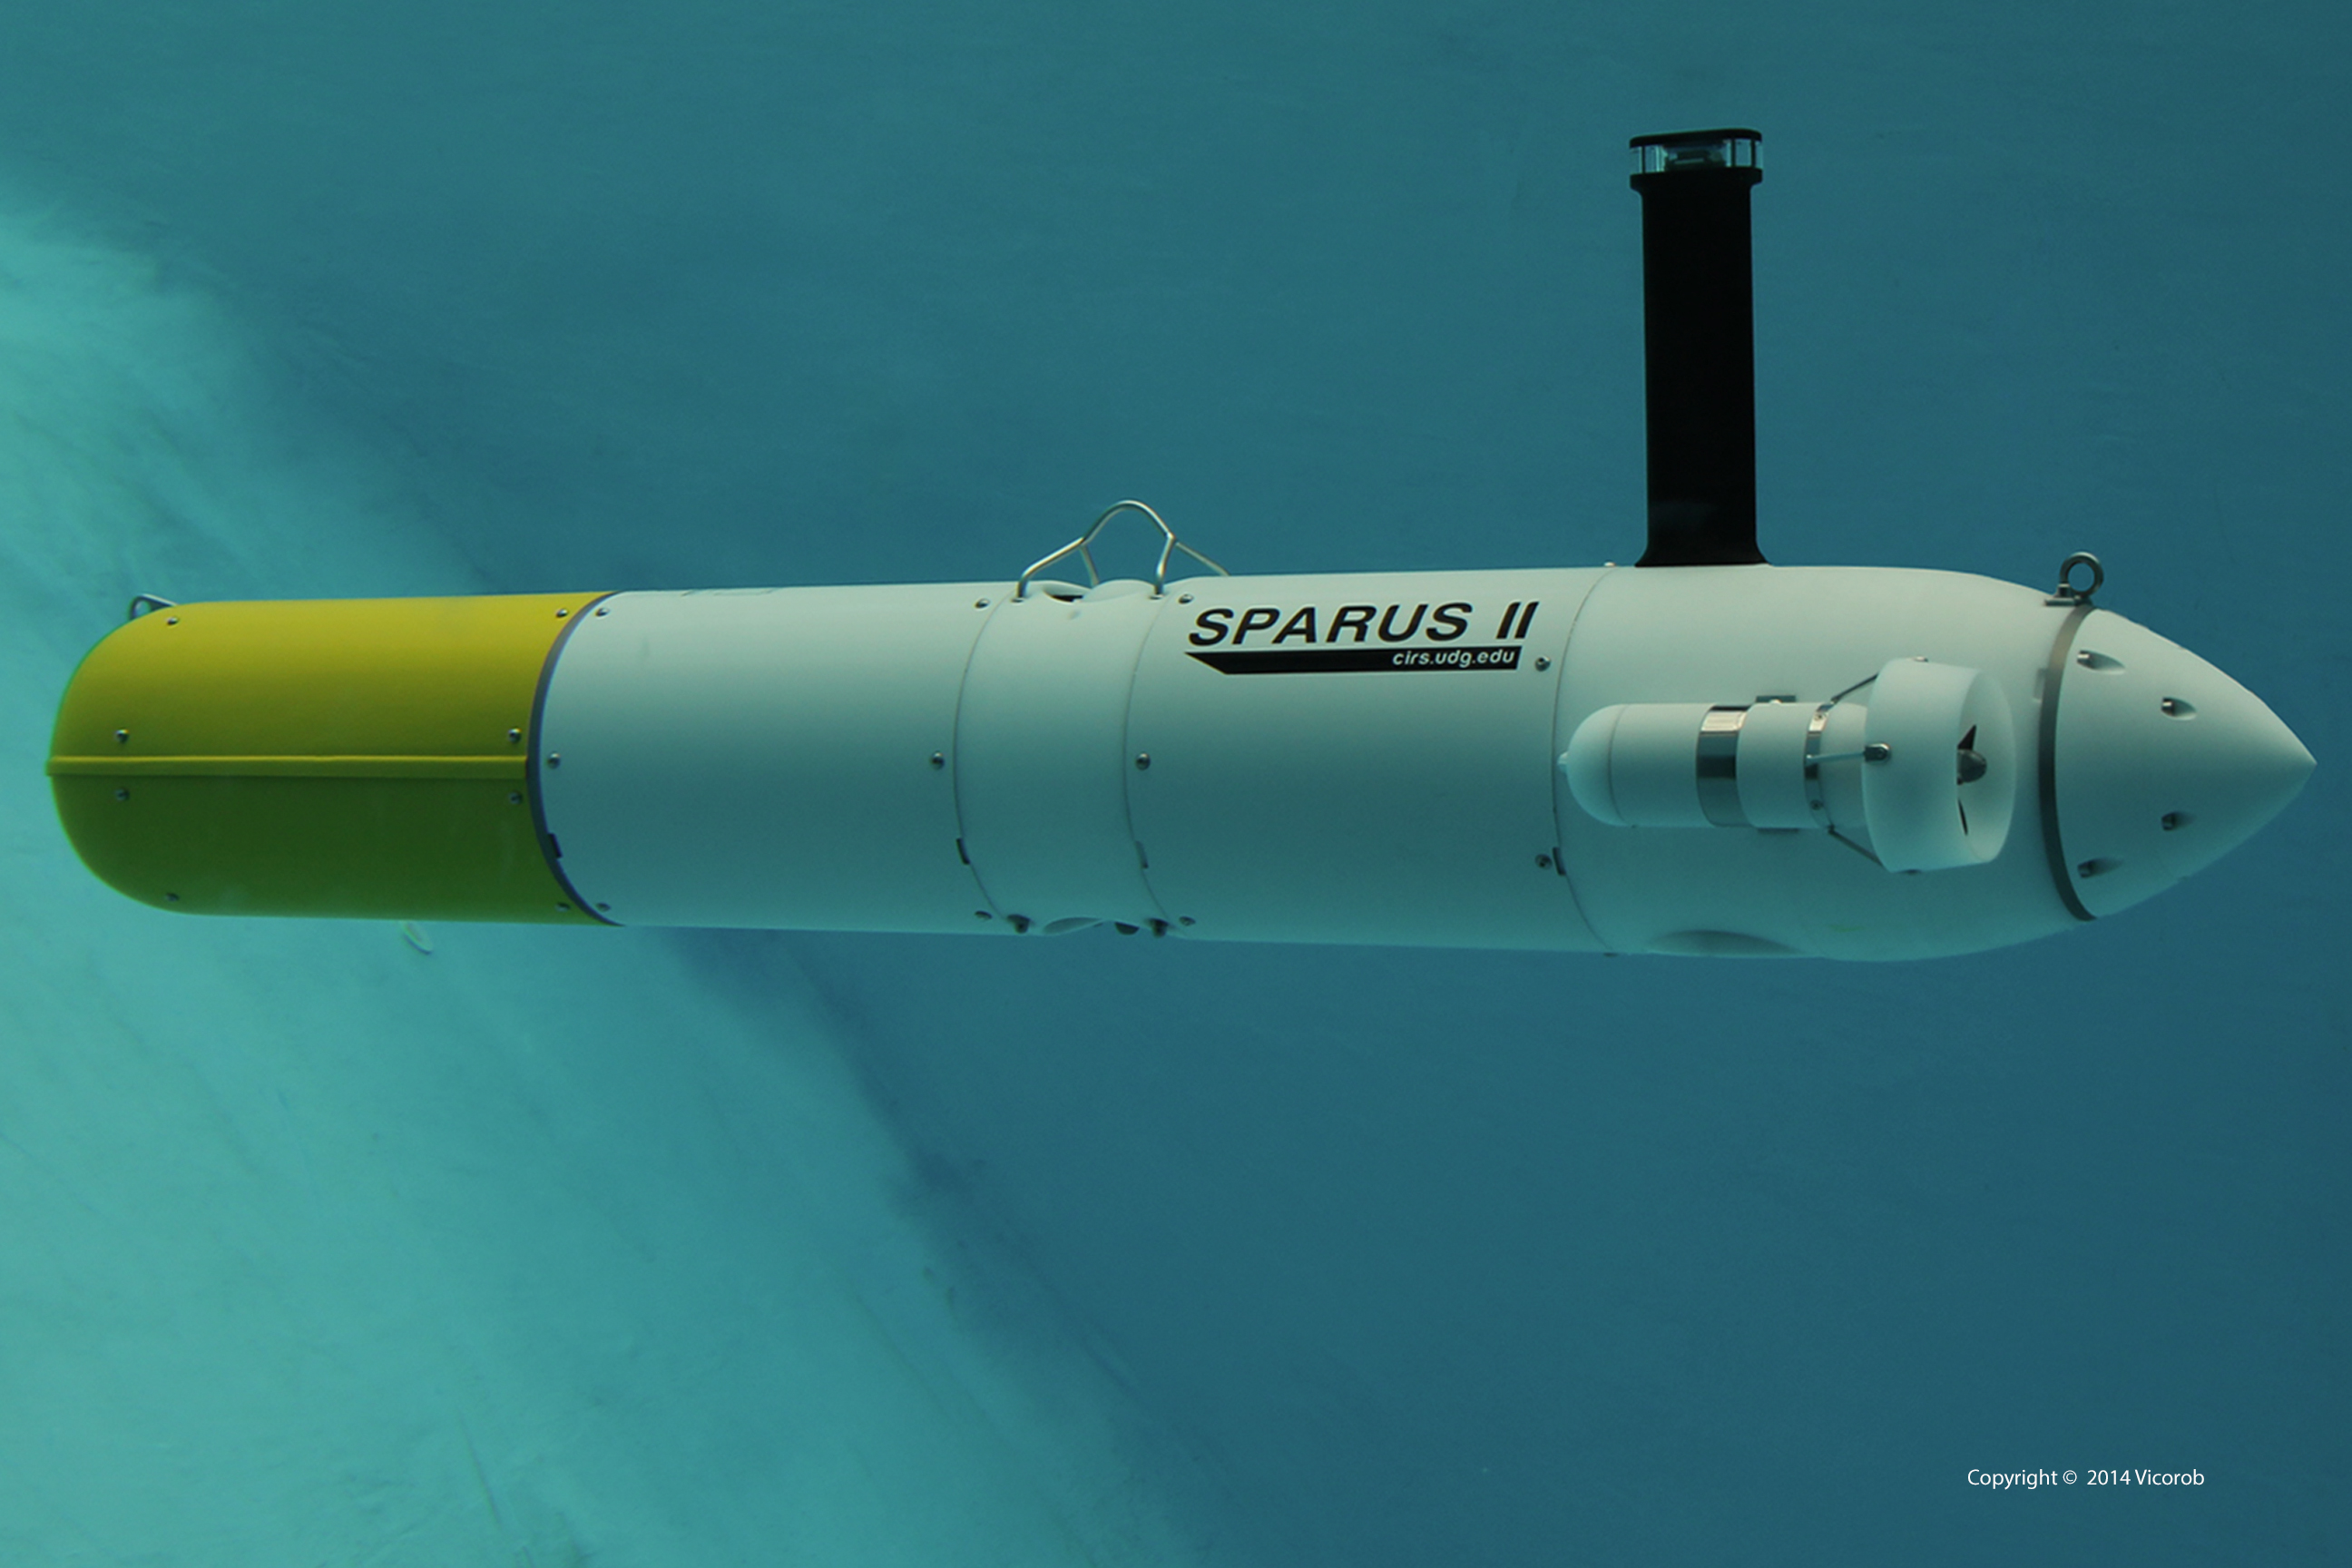
\includegraphics[width=.65\linewidth]{Sparus2FullReal}}\\
    \subfloat[Top view]
    {\label{fig:Sparus2FullTop}
    \includegraphics[width=.65\linewidth]{Sparus2FullTop}} \\%\quad
    \subfloat[Bottom view]
    {\label{fig:Sparus2FullBottom}%
     \includegraphics[width=.65\linewidth]{Sparus2FullBottom}}\\
    \subfloat[Lateral view]
    {\label{fig:Sparus2FullLateral}
    \includegraphics[width=.65\linewidth]{Sparus2FullLateral}}\\ %\quad
    \subfloat[3D view]
    {\label{fig:Sparus2Full3D}%
     \includegraphics[width=.65\linewidth]{Sparus2Full3D}}
    \caption[Sparus~II AUV: top, bottom, lateral and 3D views, and its hardware
    elements.] 
    {Sparus~II AUV: top, bottom, lateral and 3D views. Different hardware parts
    can be observed, including the thrusters (1,2), the acoustic modem (3), the
    Wi-Fi and GPS (4), as well as interoceptive and exteroceptive sensors such
    as the DVL (5), side-scan sonar (6), mechanically-scanning imaging sonar
    (7), single-beam echosounders (8), multibeam sonar (9), and an optical
    camera (10).}
    \label{fig:Sparus2FullViews}
\end{figure}

In what software concerns, the Sparus~II \ac{AUV} is controlled through the
\acf{COLA2}~\cite{Palomeras2012}, which is a control architecture that is
completely integrated with the \acf{ROS}. Besides operating aboard real robots,
\ac{COLA2} can interact with the \acf{UWSim}~\cite{Prats2012}, which can import
\ac{3D} environment models and simulate the vehicle's sensors and dynamics with
high fidelity. Furthermore, the use of \ac{ROS} allows to easily integrate third
party tools, such as the \acf{OMPL} that offers a convenient framework that can
be adapted to specific path/motion planning problems~\cite{Sucan2012}.

% \begin{figure}[htbp]
% 	\centering
% 	\includegraphics[width=.85\linewidth]{MicronAperture} 
% 	\caption{\hl{Micron} Aperture.}
% 	\label{fig:MicronAperture}
% \end{figure}

\section{AsterX AUV}

The AsterX is a torpedo-shaped \ac{AUV} from the \acf{Ifremer}. This vehicle is
based on the Explorer~3000 \ac{AUV}, which is built by \ac{ISE}, from Canada.
The vehicle is rated for depths up to $3000 m$, and is equipped with one back
propulsion motor, three aft steering planes, and two fore planes. Similarly as
the Sparus~II, AsterX is equipped with a navigation sensor suite that includes a
pressure sensor, a \ac{DVL}, an \ac{IMU} and a GPS to receive position fixes
while at surface. It also has an acoustic modem, and a Wi-Fi antenna. This
\ac{AUV} also includes a modular payload area in the front, which may carry
different sensors, \eg a multibeam sonar. Figure~\ref{fig:AsterXFullViews}
depicts the AsterX \ac{AUV} at sea surface, and a schematic with its main inner
hardware devices distribution.

\begin{figure}[htbp]
    \myfloatalign
    \subfloat[AsterX \ac{AUV} at sea surface during in-water trials]
    {\label{fig:AsterXFullReal}%
     \includegraphics[width=.65\linewidth]{AsterXFullReal}}\\
%     \subfloat[Top view]
%     {\label{fig:AsterXFullTop}
%     \includegraphics[width=.65\linewidth]{AsterXFullTop}} \\%\quad
    \subfloat[Lateral view]
    {\label{fig:AsterXFullLateral}
    \includegraphics[width=.65\linewidth]{AsterXFullLateral}}\\ %\quad
    \caption[AsterX AUV at sea surface and its lateral view with a description of the
    different hardware elements.]
    {AsterX AUV at sea surface and its lateral view with a description of the
    different hardware elements.}
    \label{fig:AsterXFullViews}
\end{figure}

On the other hand, the AsterX's software architecture is composed of
three main functional blocks (see Fig.~\ref{fig:HighLevelControArch}).  Firstly,
the \ac{AUV} low-level controller, also referred as \textit{frontseat}, guides
the vehicle using the \ac{ACE} middleware. This controller is executed over QNX
operating system, thus guaranteeing real-time computation constraints.
Furthermore, this functional block also handles the vehicle's navigation and
safety routines. Secondly, the \textit{backseat} controller extends the
vehicle's capabilities and applications by easing the implementation of
high-level routines, such as algorithms for path/motion planning, path-tracking,
and docking. These routines can directly send low-level control setpoints. This
functional block has its own dedicated computer that works under the \ac{ROS}
(over Linux). Finally, the \textit{payload} controller acts as a bidirectional
interface between the interoceptive and exteroceptive sensors, and, on the other
hand, both the \textit{frontseat} and \textit{backseat} controllers.

\begin{figure}[htbp] %  figure placement: here, top, bottom, or page
\centering
	\includegraphics[width=.7\linewidth]{AsterX-Software-Architecture}
\caption[AsterX AUV software architecture.]
{AsterX \ac{AUV} software architecture}
\label{fig:HighLevelControArch}
\end{figure}


%********************************************************************
% Other Stuff in the Back
%*******************************************************
\cleardoublepage\include{0_frontmatter/Bibliography}
%\cleardoublepage%*******************************************************
% Declaration
%*******************************************************
\refstepcounter{dummy}
\pdfbookmark[0]{CERTIFICAT DE DIRECCIO DE TESI}{Certificat de Direccio de Tesi}
\chapter*{Certificat de Direcció de Tesi}
\thispagestyle{empty}

Dr. Pere Vilà Talleda and Dr. Lluís Fàbrega Soler, del Departament 
d’Arqui-tectura i Tecnologia de Computadors de la Universitat de Girona,

\bigskip

DECLAREM:

\bigskip

\noindent Que el treball titulat \myTitle, que presenta \myName per a l’obtenció
del títol de doctor, ha estat realitzat sota la nostra direcció i que compleix els requisits
per poder optar a Menció Internacional.

\bigskip

I, perquè així consti i tingui els efectes oportuns, signem aquest
document.

\bigskip
 
\noindent\textit{Girona, Juliol 2018}

\smallskip

\begin{flushright}
    \begin{tabular}{m{5cm} m{1.5cm} m{5cm}}
        \\ \cline{1-1} \cline{3-3}
        \centering\mySupervisor& &\centering\myOtherSupervisor \\
    \end{tabular}
\end{flushright}

%\cleardoublepage\include{0_frontmatter/Colophon}
%********************************************************************
% Game Over: Restore, Restart, or Quit?
%*******************************************************
\end{document}
% ********************************************************************